\chapter{Objective 5}
Our heroes were super excited for the Talks lobby. As they started wandering around, they noticed that right behind {\color{codegreen}Chimney Scissorsticks} is a red lightbulb. He mentioned something about greeting cards, which
Grinch liked so he checked it out. It looked like a cute Image Generator, so Grinch went ahead and stored some images in his laptop to send to his colleagues.

Walking around, they bumped into {\color{codegreen}Bushy Evergreen}. He had trouble opening a door. Sure, Grinch could help.

\subsection{The door binary}
This is fairly trivial, because we can use \textit{strings}
\begin{minted}{bash}
elf@7ffd5dda212e ~ $ strings door | grep pass
/home/elf/doorYou look at the screen. It wants a password. You roll your eyes - the
password is probably stored right in the binary. There's gotta be a
Be sure to finish the challenge in prod: And don't forget, the password is "Op3nTheD00r"
Beep boop invalid password
elf@7ffd5dda212e ~ $ ./door
You look at the screen. It wants a password. You roll your eyes - the
password is probably stored right in the binary. There's gotta be a
tool for this...

What do you enter? > Op3nTheD00r
Checking......

Door opened!
\end{minted}

Generally, it is a bad idea to hardcode credentials, whether you do it in binary files or in scripts. Just don't do it.
\subsection {Lights binary}
Grinch went in the room and it was dark, so he went back and started helping the poor elf with his password problems.
Apparently, not only he has issues with his lights, he needs to evaluate an RFID door.

Per his hint, we need to set the password as the name.

\begin{minted}{bash}
# Alter the lights.conf file
elf@8a8c7a9fa846 ~/lab $ cat lights.conf
password: E$ed633d885dcb9b2f3f0118361de4d57752712c27c5316a95d9e5e5b124
name: E$ed633d885dcb9b2f3f0118361de4d57752712c27c5316a95d9e5e5b124
elf@8a8c7a9fa846 ~/lab $ ./lights

The speaker unpreparedness room sure is dark, you're thinking (assuming
you've opened the door; otherwise, you wonder how dark it actually is)

You wonder how to turn the lights on? If only you had some kind of hin---

 >>> CONFIGURATION FILE LOADED, SELECT FIELDS DECRYPTED: /home/elf/lab/lights.conf

---t to help figure out the password... I guess you'll just have to make do!

The terminal just blinks: Welcome back, Computer-TurnLightsOn # Passwd

What do you enter? >
\end{minted}

Grinch opened up the original binary
\begin{minted}{bash}
elf@2d7c99d71386 ~ $ ./lights
The speaker unpreparedness room sure is dark, you're thinking (assuming
you've opened the door; otherwise, you wonder how dark it actually is)

You wonder how to turn the lights on? If only you had some kind of hin---

 >>> CONFIGURATION FILE LOADED, SELECT FIELDS DECRYPTED: /home/elf/lights.conf

---t to help figure out the password... I guess you'll just have to make do!

The terminal just blinks: Welcome back, elf-technician

What do you enter? > Computer-TurnLightsOn
Checking......

Lights on!
\end{minted}
and there was light.

\subsection{Vending Machine Binary}
We know from the hints, the following:
\begin{itemize}
  \item The elf is telling us to try 8 Characters
  \item By inspecting the config file, the range is A-Z, a-z, 0-9
  \item If we try more than 8 characters, i.e. AAAAAAAAA the 9th character encodes like the 1st thus the algorithm repeats itself.
  \item The password is 10 characters long.
  \item The elf told us that if we remove the file, we can set our own password and see how it's "encrypted"
\end{itemize}

There are many solutions and Grinch was lucky because he figured the password without going through the whole range of characters.
But in reality, a solution would look more like
\begin{itemize}
  \item Remove the vending-machine.json file
  \item For every one of 0123456789abcdefghijklmnopqrstuvwxyzABCDEFGHIJKLMNOPQRSTUVWXYZ, put it as input, e.g. AAAAAAAA
  \item Store result
  \item Inspect to figure out the password
\end{itemize}

Grinch though started with capitals first. Reaching C, he realized that the first and fifth letter \footnote{Remember, we are inputting 8-blocks of the same character.} of the password was C and the password was 10 characters long.
CandyCanes is 10 characters. He tried it, and he was super excited that he skipped on writing an algorithm, until he hit a road block. He was missing the last character. After a little trial and error, he went ahead and consulted Cindy Lou.

- Maybe try some numbers?

Indeed, the password was CandyCane1.

\begin{minted}{bash}
elf@94dc698810f2 ~ $ ./vending-machines
The elves are hungry!

If the door's still closed or the lights are still off, you know because
you can hear them complaining about the turned-off vending machines!
You can probably make some friends if you can get them back on...

Loading configuration from: /home/elf/vending-machines.json

I wonder what would happen if it couldn't find its config file? Maybe that's
something you could figure out in the lab...

Welcome, elf-maintenance! It looks like you want to turn the vending machines back on?
Please enter the vending-machine-back-on code > CandyCane1
Checking......

Vending machines enabled!!
\end{minted}

He was super excited. After learning from the elf that Proxmark could scan other badged he rushed in the room to get candy off of the candy machine. Sadly, the candy machine was not working. Meanwhile, Cindy Lou found out another item they were missing, a button.

Cindy stopped him right there.

- You know, we may have to go around and scan elves to get somewhere that we are not allowed to.

- Yeah, well, good thing Shinny Uppatree is highly appreciated by Santa. I'd scan him.

\subsection {Snowball Machine}

Grinch was feeling betrayed, the vending machine didn't work and he really wanted that candy. On the other hand, Cindy Lou was already eye-balling that Snowball machine.
Maybe we can win it, somehow. She chatted with {\color{codegreen}Tangle Coalbox}. He was just hanging there by the Snowball Machine in the Speaker Unpreparedness room. He hinted that maybe the machine was using a PRNG that wasn't cryptographically secure.

- Maybe, if I find a way to find the seeds, I can predict the state.

She went ahead and watched that talk, and grabbed the source code. By looking at the game, she realized that she could possibly game it and win.
She inspected the source code of the game in impossible and she saw that the game comments out (in HTML) the rejected seeds. Maybe if she fed them in that script, she could win that game and get even more hints. While Grinch was focused on food, she was focused on hints.
Her gameplan was:
\begin{itemize}
  \item Grab the seeds from the source code.
  \item Feed them into the script so that the MT is in sync with the seeds produced by the snowball machine.
  \item Open the game in another tab and put in the next seed produced by her script in the easiest level.
  \item Figure out the enemy positions
  \item Win in impossible.
\end{itemize}
She figured it would be easy to verify. If the positions between the two games matched, she'd be right.

She cobbled together a script
\begin{minted}{python}
#!/usr/bin/env python3

import random

class mt19937():
    u, d = 11, 0xFFFFFFFF
    s, b = 7, 0x9D2C5680
    t, c = 15, 0xEFC60000
    l = 18
    n = 624

    def my_int32(self, x):
        return(x & 0xFFFFFFFF)

    def __init__(self, seed):
        w = 32
        r = 31
        f = 1812433253
        self.m = 397
        self.a = 0x9908B0DF
        self.MT = [0] * self.n
        self.index = self.n + 1
        self.lower_mask = (1 << r) - 1
        self.upper_mask = self.my_int32(~self.lower_mask)
        self.MT[0] = self.my_int32(seed)
        for i in range(1, self.n):
            self.MT[i] = self.my_int32((f * (self.MT[i - 1] ^ (self.MT[i - 1] >> (w - 2))) + i))

    def extract_number(self):
        if self.index >= self.n:
            self.twist()
            self.index = 0
        y = self.MT[self.index]
        # this implements the so-called "tempering matrix"
        # this, functionally, should alter the output to
        # provide a better, higher-dimensional distribution
        # of the most significant bits in the numbers extracted
        y = y ^ ((y >> self.u) & self.d)
        y = y ^ ((y << self.s) & self.b)
        y = y ^ ((y << self.t) & self.c)
        y = y ^ (y >> self.l)
        self.index += 1
        return self.my_int32(y)

    def twist(self):
        for i in range(0, self.n):
            x = (self.MT[i] & self.upper_mask) + (self.MT[(i + 1) % self.n] & self.lower_mask)
            xA = x >> 1
            if(x % 2) != 0:
                xA = xA ^ self.a
            self.MT[i] = self.MT[(i + self.m) % self.n] ^ xA

def untemper(y):
    y ^= y >> mt19937.l
    y ^= y << mt19937.t & mt19937.c
    for i in range(7):
        y ^= y << mt19937.s & mt19937.b
    for i in range(3):
        y ^= y >> mt19937.u & mt19937.d
    return y
# Paste your seeds here.
comments = """
    3265172653 - Not random enough
    1042856531 - Not random enough
"""
def parse_comments():
    data = comments.split('\n')[1:-1]
    numbers = []
    for comment in data:
        numbers.append(int(comment.strip().split('-')[0].strip()))
    return numbers

if __name__ == "__main__":
    numbers = parse_comments()

    # create our own version of an MT19937 PRNG.
    myprng = mt19937(0)

    print("Feeding %i numbers from comments var.\nWe'll use those values to create a clone of the current state of Python's built-in PRNG..." % (mt19937.n))
    for i in range(mt19937.n):
        myprng.MT[i] = untemper(numbers[i])
    print("Now, we'll test the clone...")
    print("\nOur clone (pick the first number)")
    for i in range(5):
        r2 = myprng.extract_number()
        print("%10.10i" % (r2))
\end{minted}
... Sure enough she won. {\color{codegreen}Tangle Coalbox} gave them some hints that baffled our heroes.
\subsection{Santavator... Again}
Having completed everything in that floor, our heroes decided to head back to the santavator. with minor adjustments, they figured they could visit different floors. After all, they had the missing button and the red lamp.
\begin{figure}[h!]
  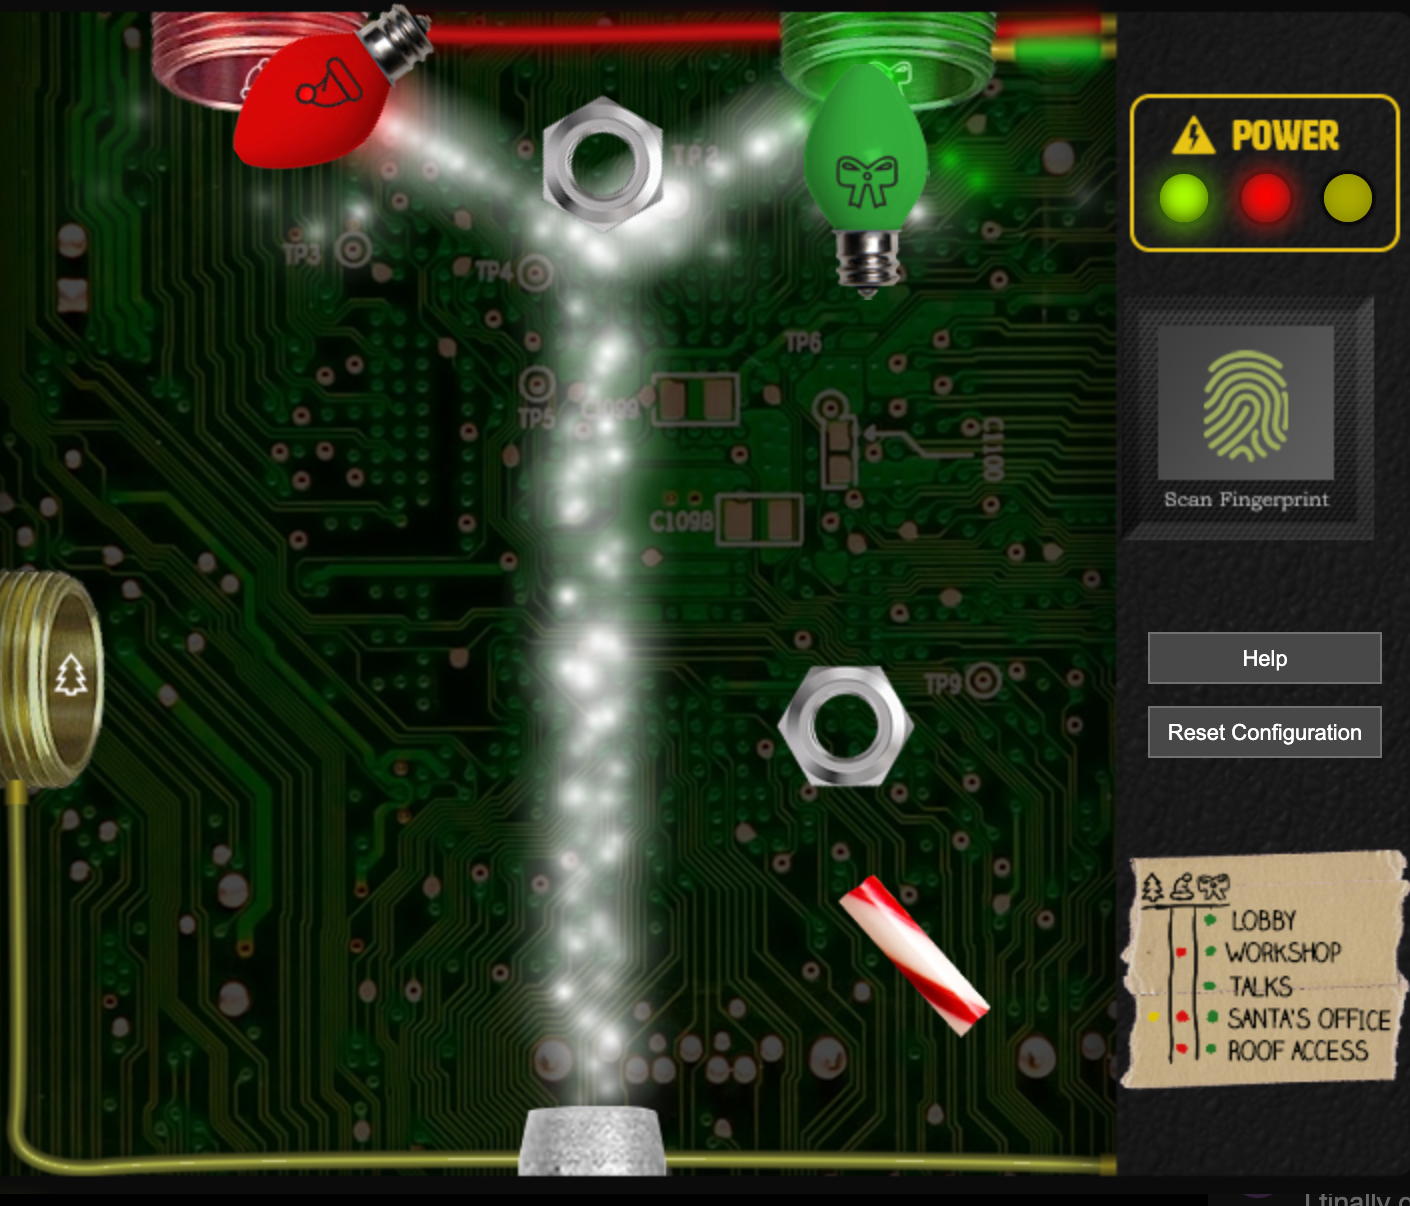
\includegraphics[scale=0.5]{santavator-2}
  \caption{Power to red and green line.}
\end{figure}

\section{Workshop}
Our heroes decided to go to the workshop and explore further.
In the Wrapping room, they found a \textit{large marble}.

\subsection{Sort O Matic}
{\color{codegreen}Minty Candycane} asked for help with some regular expressions. Grinch remembered the time he managed to pwn a whole company because their regex was dreadful so he decided to give it a try.
\begin{itemize}
  \item Matches at least one digit: \textit{\textbackslash d}
  \item Match three a-z ignoring case: \textit{[A-Za-z]\{3\}}
  \item Match 2 lowercase chars or digits: \textit{[a-z0-9]{2}}
  \item Match any 2 char but not A-L 1-5: \textit{[\^{}A-L1-5]\{2\}}
  \item Match 3 or more digits only: \textit{[0-9]\{3,\}\$}
  \item Match multiple HH:MM:SS: \textit{\^{}([0-5]\d):([0-5]\d):([0-5]\d)\$}
  \item Match MAC Address: \textit{\^{}([0-9A-Fa-f]\{2\}[:])\{5\}([0-9A-Fa-f]\{2\})\$}
  \item Match multiple day month year formats : \begin{Verbatim}[fontsize=\small,frame=single]
^(0?[1-9]|[12]\d|30|31)[/\.-](0[1-9]|1[0-2])[/\.-](\d{4}|\d{2})$
\end{Verbatim}
\end{itemize}

And this wraps up Sort-O-Matic. The elf is giving us some hints about the Splunk challenge.

On the next room, there's a challenge that, again, our heroes are not allowed to touch. Also, \textit{proxmark} and \textit{rubber ball} are in this room.

\subsection{Unlocking HID door}
We have already seen that there is a locked door next to {\color{codegreen}Minty Candycane} and based on the objective, we need to find a valid RFID tag. We already know from {\color{codegreen}Fitzy Shortstack} that {\color{codegreen}Shinny Uppatree} is trusted. Let's get close to him and scan his badge (he's located in the castle approach area).
An alternative approach is to scan two random badges and then bruteforce the ending bytes until we are in.

Anyway, Grinch decided to scan that specific elf, so...

\begin{minted}{bash}
[magicdust] pm3 --> lf hid read

#db# TAG ID: 2006e22f13 (6025) - Format Len: 26 bit - FC: 113 - Card: 6025
\end{minted}

Now that we have his badge, our heroes headed back to the Workshop.
\begin{minted}{bash}
[magicdust] pm3 --> lf hid sim -r 2006e22f13
\end{minted}

Our heroes opened that locked door.
